\documentclass{beamer}
\usepackage{booktabs}
\usepackage{ctex}
\usepackage{graphicx}
\usepackage{listings}
\usepackage{hyperref}
\usepackage{ulem}

\title{Number Theory}
\author{whx1003}
\date{2024 年 8 月 16 日}

\usetheme{default}
\geometry{paperheight=11.0cm,paperwidth=16.0cm}
\setbeamertemplate{background}{
\includegraphics[height=\paperheight]{images/bg.png}}
\addtobeamertemplate{block begin}{\pgfsetfillopacity{0.75}}{\pgfsetfillopacity{1}}
\addtobeamertemplate{block alerted begin}{\pgfsetfillopacity{0.75}}{\pgfsetfillopacity{1}}
\addtobeamertemplate{block example begin}{\pgfsetfillopacity{0.75}}{\pgfsetfillopacity{1}}

\definecolor{uibred}  {HTML}{db3f3d}
\definecolor{uibblue} {HTML}{4ea0b7}
\definecolor{uibgreen}{HTML}{789a5b}
\definecolor{uibgray} {HTML}{d0cac2}
\definecolor{uiblink} {HTML}{00769E}
\setbeamercolor{block body} {bg = uibgray}
\setbeamercolor{block title}{fg = white,bg = uibblue}

\usefonttheme{serif}
\AtBeginDocument{
    \DeclareSymbolFont{pureletters}{OML}{cmm}{m}{it}
    \SetSymbolFont{pureletters}{bold}{OML}{cmm}{bf}{it}
}
\hypersetup{
    hidelinks,
    colorlinks=true,
    urlcolor=blue
}

\newcommand{\nl}{\\\hspace*{\fill}\\}

\lstset{
    backgroundcolor=\color{white},      % choose the background color
    basicstyle=\footnotesize\ttfamily,  % size of fonts used for the code
    columns=fullflexible,
    tabsize=4,
    breaklines=true,               % automatic line breaking only at whitespace
    captionpos=b,                  % sets the caption-position to bottom
    commentstyle=\color{green}, % comment style
    escapeinside={\%*}{*)},        % if you want to add LaTeX within your code
    keywordstyle=\color{blue},     % keyword style
    stringstyle=\color{mymauve}\ttfamily,  % string literal style
    frame=none,
    rulesepcolor=\color{red!20!green!20!blue!20},
    % identifierstyle=\color{green},
    language=c++,
}

\begin{document}
    \maketitle

    \begin{frame}{Preface}
        今天的主要内容是一些基本的数论知识, 包括
        \begin{itemize}
            \item 常见的数论函数
            \item 某些神秘的数论公式
            \item 筛法
        \end{itemize}
    \end{frame}

    \begin{frame}{数论函数}
        \begin{itemize}
            \item 数论函数: 定义域为正整数的函数, OI 中常见的数论函数大部分的值域是整数.
            \item 完全积性函数: 对任意正整数 $n,m$ 均有 $f(nm)=f(n)f(m)$ 的函数.
            \item 积性函数: 对满足 $n\perp m$ 的正整数 $n,m$ 有 $f(nm)=f(n)f(m)$ 的函数.
            \item 质因数分解: 每个正整数 $n$ 总能唯一地表示为
            $$
            n=\prod_{i=1}^m p_i^{r_i}
            $$
            
            的形式, 其中 $p_i$ 为互不相同的质数, $r_i\geq 1$.
        \end{itemize}
        推论 1: 积性函数 $f$ 一定满足 $f(1)=1$.\nl
        推论 2: 通过质数处点值可以唯一确定完全积性函数; 通过全部 $p^k$ 处点值可以唯一确定积性函数.
    \end{frame}

    \begin{frame}{Dirchlet 卷积}
        \begin{itemize}
            \item Dirchlet 卷积: 对两个数论函数 $f,g$, 定义它们的 Dirchlet 卷积
            $$
            (f\otimes g)(n)=\sum_{d\mid n}f(d)g(n/d)=\sum_{xy=n}f(x)g(y).
            $$
        \end{itemize}
        Dirchlet 卷积是 OI 中数论的最重要概念, 他有如下的优良性质:
        \begin{itemize}
            \item 交换律: $f\otimes g=g\otimes f$;
            \item 结合律: $f\otimes g\otimes h=f\otimes(g\otimes h)$;
            \item 单位元: 取 $\varepsilon(n)=[n=1]$, 则对任意数论函数 $f$ 都有 $f\otimes\varepsilon=\varepsilon\otimes f=f$;
            \item 两个积性函数的 Dirchlet 卷积仍是积性函数;
            \item 积性函数的 Dirchlet 逆仍是积性函数.
        \end{itemize}
        Dirchlet 逆的概念见下一页
    \end{frame}

    \begin{frame}{Dirchlet 卷积}
        \begin{block}{计算 Dirchlet 卷积}
            给出数论函数 $f,g$ 在 $1\dots n$ 上的点值, 计算 $f\otimes g$ 在 $1\dots n$ 上的点值.
        \end{block}
        \pause
        直接暴力计算即可, 复杂度是
        $$
        \sum_{h=1}^n\#\{x\mid h\}=\sum_{x=1}^n\sum_{h=1}^n[x\mid h]=\sum_{x=1}^n\left\lfloor\frac nx\right\rfloor=\mathcal O(n\log n).
        $$
        \pause
        \begin{block}{计算 Dirchlet 逆}
            给出数论函数 $f$ 在 $1\dots n$ 上的点值, 求一个数论函数 $g$ 满足 $f\otimes g=\varepsilon$. 保证 $f(1)\neq 0$.
        \end{block}
        \pause
        首先有 $g(1)=\frac 1{f(1)}$. 对 $n\geq 2$ 我们有
        \begin{align*}
            (f\otimes g)(n)=\varepsilon(n)=0&\implies\sum_{d\mid n}f(d)g(n/d)=0\\
            &\implies g(n)=-\frac 1{f(1)}\sum_{d\mid n,d>1}f(d)g(n/d)
        \end{align*}
        暴力计算的复杂度也是 $\mathcal O(n\log n)$.
    \end{frame}

    \begin{frame}{Dirchlet 卷积}
        \begin{block}{试看看!}
            考虑积性函数 $1(n)\equiv 1$, 计算它的 Dirchlet 逆.
        \end{block}
        \pause
        不妨记 $\mu:=1^{-1}$, 我们来简单计算一下前几项:
        \begin{center}
            \begin{tabular}{c|cccccccccccccccc}
                \toprule
                      & $1$ & $2$  & $3$  & $4$ & $5$  & $6$ & $7$  & $8$ & $9$ & $10$ & $11$ & $12$ & $13$ & $14$ & $15$ & $16$\\
                \hline
                $\mu$ & $1$ & $-1$ & $-1$ & $0$ & $-1$ & $1$ & $-1$ & $0$ & $0$ & $1$  & $-1$ &  $0$ & $-1$ &  $1$ &  $1$ &  $0$\\
                \bottomrule
            \end{tabular}\\
        \end{center}
        简单观察一下规律:
        \begin{itemize}
            \item 在 $n=p$ 处 $\mu(p)=-1$;
            \item 在 $n=pq$ 处 $\mu(pq)=1$;
            \item 在 $n=p^k(k>1)$ 处 $\mu(p^k)=0$;
        \end{itemize}
        我们之前提到过, 积性函数的 Dirchlet 逆仍积性, 且通过所有 $p^k$ 处的点值可以唯一确定一个积性函数, 因此不难推理出
        $$
        \mu(n)=\begin{cases}
        (-1)^{\#\text{prime factors of }n} & n\text{ is square free}\\
        0 & \text{otherwise}
        \end{cases}
        $$

        这是可以归纳证明的. 实际上 $\mu$ 就是大名鼎鼎的 M\"obius 函数.
    \end{frame}

    \begin{frame}{Dirchlet 卷积}
        \begin{block}{试看看!}
            考虑积性函数 ${\rm id}(n)=n$, 计算 Dirchlet 卷积 $\mu\otimes{\rm id}$.
        \end{block}
        \pause
        不妨记 $\varphi:=\mu\otimes{\rm id}$, 我们来简单计算一下前几项:
        \begin{center}
            \begin{tabular}{c|cccccccccccccccc}
                \toprule
                          & $1$ & $2$ & $3$ & $4$ & $5$ & $6$ & $7$ & $8$ & $9$ & $10$ & $11$ & $12$ & $13$ & $14$ & $15$ & $16$\\
                \hline
                $\varphi$ & $1$ & $1$ & $2$ & $2$ & $4$ & $2$ & $6$ & $4$ & $6$ & $4$  & $10$ &  $4$ & $12$ &  $6$ &  $8$ &  $8$\\
                \bottomrule
            \end{tabular}\\
        \end{center}
        简单观察一下规律:
        \begin{itemize}
            \item 在 $n=p$ 处 $\varphi(p)=p-1$;
            \item 在 $n=p^k(k>1)$ 处 $\varphi(p^k)=(p-1)p^{k-1}$;
        \end{itemize}
        不难推理出
        $$
        \varphi(n)=n\prod_{i=1}^k{p_i-1\over p_i},\quad\text{where }n=\prod_{i=1}^kp_i^{r_i}
        $$

        这是可以归纳证明的. 实际上 $\varphi$ 就是大名鼎鼎的 Euler totient 函数.
    \end{frame}

    \begin{frame}{Dirchlet 卷积}
        注意到我们关于 $\mu$ 和 $\varphi$ 的定义给出两个重要等式:
        \begin{block}{$\mu$ 的数论性质}
            $$
            \sum_{d\mid n}\mu(d)=[n=1]
            $$
        \end{block}
        注意到 $\mu=1^{-1}$, 于是 $\mu\otimes 1=\varepsilon$, 从而写开即证.
        \begin{block}{$\varphi$ 的数论性质}
            $$
            \sum_{d\mid n}\varphi(d)=n
            $$
        \end{block}
        注意到 $\varphi={\rm id}\otimes\mu={\rm id}\otimes 1^{-1}$, 于是 $\varphi\otimes 1={\rm id}$, 从而写开即证.
    \end{frame}

    \begin{frame}{Dirchlet 卷积}
        至此我们已经见过了大部分常见的数论函数
        \begin{itemize}
            \item 单位元 $\varepsilon$;
            \item ${\rm id}_k(n)=n^k$, 一般记 ${\rm id}={\rm id}_1$, 记 $1(n)=I(n)={\rm id}_0(n)\equiv 1$;
            \item $\sigma_k(n)=\sum_{d\mid n}d^k$, 一般记 $d(n):=\sigma_0(n)$ 为因数个数函数;
            \item M\"obius 函数 $\mu(n)$;
            \item Euler totient 函数 $\varphi(n)$.\nl
        \end{itemize}
        它们之间有关系:
        \begin{itemize}
            \item $\mu\otimes 1=\varepsilon$;
            \item $\varphi\otimes 1={\rm id}$;
            \item $\mu\otimes{\rm id}=\varphi$;
            \item $1\otimes 1=d=\sigma_0$;
            \item $1\otimes{\rm id}_k=d=\sigma_k$;\nl
        \end{itemize}
        其中前三者是 OI 中数论的核心等式.
    \end{frame}
    
    \begin{frame}{Dirchlet 卷积}
        这里需要额外提一下 $\mu$ 和 $\varphi$ 的组合意义:\nl
        $\varphi$ 的组合意义是, $\varphi(n)$ 恰为 $1\dots n$ 之间与 $n$ 互质的数的个数. 也即
        $$
        \varphi(n)=\sum_{d=1}^n[d\perp n]
        $$

        $\varphi$ 的两种定义是可以互推的:
        \begin{align*}
            \varphi(n)&=\sum_{d=1}^n[\gcd(d,n)=1]=\sum_{d=1}^n\varepsilon(\gcd(d,n))\\
            &=\sum_{d=1}^n\sum_{k\mid\gcd(d,n)}\mu(k)=\sum_{k\mid n}\mu(k)\frac nk
        \end{align*}

        最后一式就是 Dirchlet 卷积 $\varphi=\mu\otimes{\rm id}$.
    \end{frame}

    \begin{frame}{M\"obius 反演}
        而 $\mu$ 的组合意义则和 M\"obius 反演有关:
        \begin{block}{M\"obius 反演}
            $$
            f(n)=\sum_{d\mid n}g(d)\iff g(n)=\sum_{d\mid n}f(d)\mu(n/d)
            $$
        \end{block}
        大家可以联想一下已经学过的其它反演:
        \begin{block}{子集反演}
            $$
            f_S=\sum_{T\subseteq S}g(T)\iff g_S=\sum_{T\subseteq S}(-1)^{|S|-|T|}f_T.
            $$
        \end{block}
        不难发现二者有一些相似之处: 考虑记 $S$ 为 $n$ 的所有素因数的多重集, 那么枚举因数 $d\mid n$ 实际上就是枚举了一个子多重集 $T\subseteq S$. 因此 M\"obius 反演的实质就是「子多重集反演」, 而 $\mu$ 就是这个反演的系数.
    \end{frame}
    
    \begin{frame}{线性筛}
        下一个问题是, 如何计算各种数论函数在 $1\dots n$ 上的点值. 我们从一个比较简单的问题开始
        \begin{block}{打素数表}
            给定正整数 $n$, 输出 $1\dots n$ 中的所有素数.
        \end{block}
        \pause
        \begin{itemize}
            \item 做法一: 枚举每个数 $x=1\dots n$, 每次 $\mathcal O(\sqrt x)$ 判断 $x$ 是否为素数, 总复杂度 $\mathcal O(n\sqrt n)$.\nl
            \item 做法二: 维护一个 bool 数组记录每个数是否为素数, 用全体 $x=2\dots n$ 去掉其倍数 (这就是「筛法」名字的来源), 总复杂度 $\sum_x\frac nx=\mathcal O(n\log n)$.\nl
            \item 做法三 (埃拉托斯特尼筛法, 埃氏筛): 将做法三中的全体 $x$ 改为素数 $x$, 总复杂度可以分析出 $\sum_p\frac np=\mathcal O(n\log\log n)$.\nl
            \item 做法四 (欧拉筛, 线性筛): 用每个数的\textbf{最小}的质因数筛去它. 复杂度 $\mathcal O(n)$.
        \end{itemize}
    \end{frame}

    \begin{frame}[fragile]{线性筛}
        线性筛的具体做法是:
        \begin{lstlisting}
vector<int> linear_sieve(int n) {
    vector<int> is_prime(n + 1, true), primes;
    for (int i = 2; i <= n; ++i) {
        if (is_prime[i]) primes.push_back(i);
        for (int p : primes) {
            if (i * p > n) break;
            is_prime[i * p] = false;
            if (i % p == 0) break;
        }
    }
    return primes;
}\end{lstlisting}
        简单分析一下复杂度和正确性:
        \begin{itemize}
            \item 正确性: 考虑每个合数 $n$ 的最小质因数 $p$, 那么 $n/p$ 一定没有 $<p$ 的因数. 于是在我们的循环中, 当 $i=n/p$ 时, 在 $p$ 之前的素数上不会 break, 于是一定可以筛掉 $n$.
            \item 复杂度: 如果 $p$ 不是 $n$ 的最小质因数, 那么 $n/p$ 就有比 $p$ 更小的质因数 $q$. 于是在我们的循环中, 当 $i=n/p$ 时, 在 $q$ 处就会 break, 那么就不会再次筛掉 $n$.
        \end{itemize}
        于是我们可以断言, 每个合数恰被筛去了一次, 于是其正确性和复杂度均有所保证.\nl
    \end{frame}

    \begin{frame}[fragile]{线性筛}
        \begin{block}{计算 $\mu$ 和 $\phi$}
            计算 $\mu$ 和 $\phi$ 在 $1\dots n$ 上的点值.
        \end{block}
        \pause
        我们来修改之前的线性筛素数的代码:
        \begin{lstlisting}
for (int i = 2; i <= n; ++i) {
    if (is_prime[i]) {
        primes.push_back(i);
        mu[i] = -1, phi[i] = i - 1;
    }

    for (int p : primes) {
        if (i * p > n) break;
        if (i % p) {
            mu[i * p] = -mu[i];
            phi[i * p] = phi[i] * (p - 1);
        } else {
            mu[i * p] = 0;
            phi[i * p] = phi[i] * p;
            break;
        }
    }
}\end{lstlisting}
    \end{frame}

    \begin{frame}{线性筛}
        \begin{block}{计算积性函数}
            给定一个一般的积性函数 $f$, 其点值可以在 $\mathcal O(\log n)$ 时间内计算, 求它在 $1\dots n$ 处的点值.
        \end{block}
        \pause
        思路类似 $\mu$ 和 $\varphi$, 只是现在我们需要确定每个正整数的最小质因子的次数, 这也是不难实现的. 具体细节留给大家自己思考\nl
        注意到 $\leq n$ 的形如 $p^k$ 的数只有 $\mathcal O\left(n\over\log n\right)$ 个, 于是总复杂度是可以做到 $\mathcal O(n)$ 的.\nl
        关于线性筛有一个常见误区: 线性筛复杂度最低, 是否意味着运行速度一定最快? 实际上经过一些测试, 我们发现线性筛是跑不过经过一些优化的埃氏筛的. 但是线性筛的优势是它会且仅会筛去每个数一次, 因此可以比较方便地计算积性函数的点值.
    \end{frame}

    \begin{frame}{线性筛}
        \begin{block}{SPOJ PRIME1 Prime Generator}
            求 $[L,R]$ 之间的所有素数. $R\leq 10^{14},R-L+1\leq 10^6$.
        \end{block}
        \pause
        经典结论: 一个合数 $n$ 的最小质因子一定 $\leq\sqrt n$. 因此只需要先筛出 $\leq\sqrt R$ 的所有素数, 然后用每个素数筛掉它在 $[L,R]$ 之间的所有倍数即可. 筛素数是 $\mathcal O(\sqrt R)$ 的, 用素数筛 $[L,R]$ 是
        $$
        \sum_{p<\sqrt R}{R-L\over p}=\mathcal O((R-L)\log\log R)
        $$

        的, 可以通过.
    \end{frame}

    \begin{frame}{线性筛}
        \begin{block}{完全平方数}
            计算 $1\dots n$ 之间有多少个数没有平方因子. $n\leq 10^{14}$.
        \end{block}
        \pause
        相信大家小学都学过容斥原理: 用总的, 减去有一个质数的平方的, 加上有两个质数的平方的, 再减去有三个质数的平方的......
        $$
        n-\sum_p\left\lfloor n\over p^2\right\rfloor+\sum_{p_1,p_2}\left\lfloor n\over p_1^2p_2^2\right\rfloor+\cdots=\sum_{x\geq 1}\mu(x)\left\lfloor n\over x^2\right\rfloor.
        $$
        于是只需要计算 $\leq\sqrt n$ 的 $\mu$ 点值即可.\nl
        \pause
        另一个做法是, 注意到一个数无平方因子当且仅当 $\mu\neq 0\iff\mu^2=1$. 记 $f(n)$ 为 $n$ 的最大平方因子就有
        \begin{gather*}
            \mu^2(n)=[f(n)=1]=\sum_{d\mid f(n)}\mu(d)=\sum_{d^2\mid n}\mu(d)\\
            \implies\sum_{i=1}^n\mu^2(i)=\sum_{i=1}^n\sum_{d^2\mid i}\mu(d)=\sum_{d\geq 1}\mu(d)\left\lfloor n\over d^2\right\rfloor.
        \end{gather*}
    \end{frame}

    \begin{frame}{线性筛}
        \begin{block}{字符串计数}
            称字符串 $s$ 有循环节 $t$, 如果存在一个 $k\geq 2$ 使得 $s=\underbrace{t\cdots t}_k$. 现在给定字符集大小 $m$, 问有多少个长为 $n$ 的没有循环节的字符串. $m,n\leq 10^9$.
        \end{block}
        \pause
        设长为 $n$ 的答案为 $f_n$, 那么一个串一定要么没有循环节, 要么有循环节, 于是枚举循环节的长度可知
        $$
        m^n=\sum_{d\mid n}f_d\iff f_n=\sum_{d\mid n}\mu(d)m^{n/d}.
        $$

        于是只需要计算所有 $d\mid n$ 的 $\mu$, 这可以把 $n$ 提前因式分解做到. 因数个数 $d(n)$ 是比较有限的 (见下表):\\
        \begin{center}
            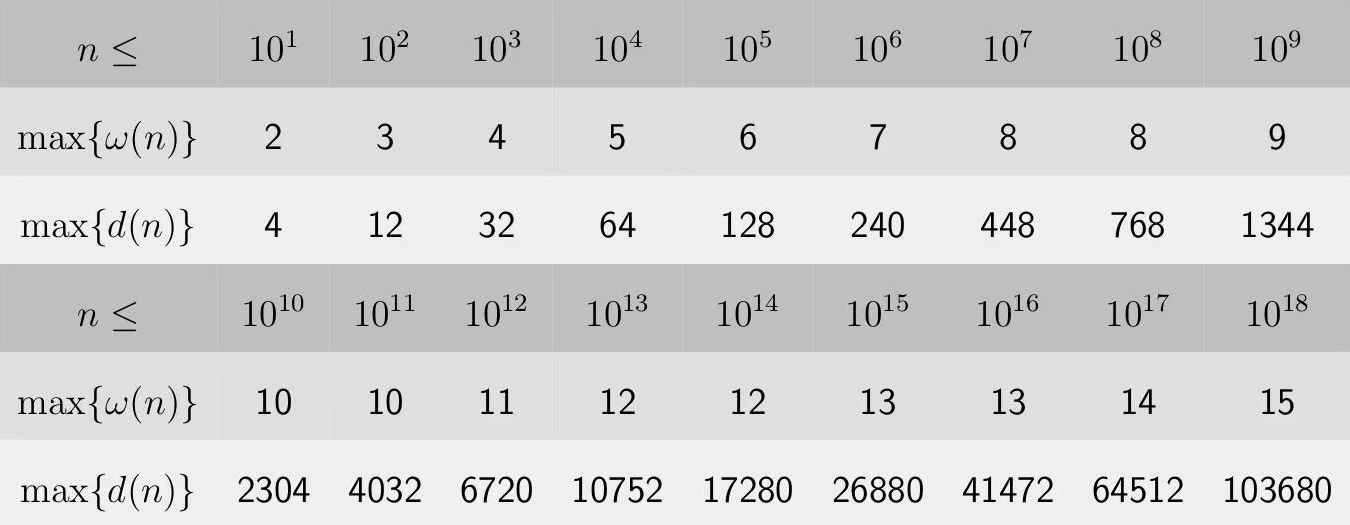
\includegraphics[scale=0.5]{images/fig1.jpg}\\
        \end{center}
    \end{frame}

    \begin{frame}[fragile]{整除分块}
        数论题中的一个常见套路是「整除分块」. 这个方法的来源是一个精巧的观察:
        \begin{block}{整除分块}
            对一个正整数 $n$, 所有形如 $\left\lfloor\frac nx\right\rfloor$ 的数的个数是什么级别?
        \end{block}
        \pause
        关键观察:
        \begin{itemize}
            \item 当 $x\leq\sqrt n$ 时, 只有 $\mathcal O(\sqrt n)$ 种不同的 $x$, 于是也只有 $\mathcal O(\sqrt n)$ 种不同的 $\left\lfloor\frac nx\right\rfloor$;
            \item 当 $x>\sqrt n$ 时, 有 $\left\lfloor\frac nx\right\rfloor\leq\sqrt n$, 于是也只有 $\mathcal O(\sqrt n)$ 种不同的 $\left\lfloor\frac nx\right\rfloor$;
        \end{itemize}
        因此不同的 $\left\lfloor\frac nx\right\rfloor$ 只有 $\mathcal O(\sqrt n)$ 个!\nl
        我们可以十分简单地枚举出这 $\mathcal O(\sqrt n)$ 个值:
        \begin{lstlisting}
for (int l = 1, r; l <= n; l = r + 1) {
    r = n / (n / l);
}\end{lstlisting}
        此时对每个 $x\in[l,r]$ 都有 $\left\lfloor\frac nx\right\rfloor=\left\lfloor\frac nl\right\rfloor$. 算法正确性的证明比较简单, 只需要注意到
        $$
        \left\lfloor\frac nl\right\rfloor=\left\lfloor\frac nr\right\rfloor\implies\left\lfloor\frac nl\right\rfloor\leq\frac nr\implies j\leq\left\lfloor n\over\lfloor n/l\rfloor\right\rfloor.
        $$
    \end{frame}

    \begin{frame}{整除分块}
        \begin{block}{典中典 \#1}
            $T$ 组询问, 每组询问给出正整数 $n$, 求
            $$
            \sum_{i=1}^n\sum_{j=1}^n\gcd(i,j)
            $$

            的值. $n\leq 10^7,T\leq 10^4$.
        \end{block}
        \pause
        我们来推一下式子. 首先我们改为枚举 $d:=\gcd(i,j)$ 就有
        $$
        =\sum_{d\geq 1}d\sum_{i=1}^n\sum_{j=1}^n[\gcd(i,j)=d]
        $$

        由于 $\gcd(i,j)=d\iff\gcd(i/d,j/d)=1$, 用 $\mu$ 来替代它就有
        $$
        =\sum_{d\geq 1}d\sum_{i=1}^{\lfloor n/d\rfloor}\sum_{j=1}^{\lfloor n/d\rfloor}[\gcd(i,j)=1]=\sum_{d\geq 1}d\sum_{i=1}^{\lfloor n/d\rfloor}\sum_{j=1}^{\lfloor n/d\lfloor}\sum_{k\mid\gcd(i,j)}\mu(k)
        $$
    \end{frame}

    \begin{frame}{整除分块}
        接下来注意到 $k\mid\gcd(i,j)\iff k\mid i\land k\mid j$. 交换求和顺序, 就有
        \begin{align*}
            &=\sum_{d\geq 1}d\sum_{k\geq 1}\mu(k)\sum_{i=1}^{\lfloor n/d\rfloor}[k\mid i]\sum_{j=1}^{\lfloor n/d\rfloor}[k\mid j]\\
            &=\sum_{d\geq 1}d\sum_{k\geq 1}\mu(k)\left\lfloor\lfloor n/d\rfloor\over k\right\rfloor\left\lfloor\lfloor n/d\rfloor\over k\right\rfloor.
        \end{align*}
        这里有一个非常好的结论: $\left\lfloor\lfloor n/x\rfloor\over y\right\rfloor=\left\lfloor n\over xy\right\rfloor$. 于是可以进一步化简:
        $$
        =\sum_{d\geq 1}d\sum_{k\geq 1}\mu(k)\left\lfloor n\over kd\right\rfloor^2
        $$

        现在我们改为枚举 $T=kd$, 于是
        $$
        =\sum_{T=1}^n\left\lfloor n\over T\right\rfloor^2\left(\sum_{kd=T}\mu(k)d\right)
        $$

        注意最后那一项其实就是 $(\mu\otimes{\rm id})(T)=\varphi(T)$, 于是
        $$
        =\sum_{T=1}^n\left\lfloor n\over T\right\rfloor^2\varphi(T)
        $$

        于是只需要维护出 $\varphi$ 的前缀和, 然后用我们之前那个整除分块的算法计算即可.
    \end{frame}

    \begin{frame}[fragile]{整除分块}
        \begin{block}{典中典 \#2}
            $T$ 组询问, 每组询问给出正整数 $n,m$, 求
            $$
            \sum_{i=1}^n\sum_{j=1}^m\gcd(i,j)
            $$

            的值. $n,m\leq 10^7,T\leq 10^4$.
        \end{block}
        \pause
        和上一个题的推导完全一致, 只是现在我们需要同时按照 $\lfloor n/T\rfloor,\lfloor m/T\rfloor$ 分块, 这也是容易实现的, 只需要每次令
        \begin{lstlisting}
            for (int l = 1, r; l <= n && l <= m; l = r + 1) {
                r = min(n / (n / l), m / (m / l));
            }\end{lstlisting}
        即可. 总的段数是 $\mathcal O(\sqrt n+\sqrt m)$ 的.
    \end{frame}

    \begin{frame}{整除分块}
        \begin{block}{典中典 \#3}
            $T$ 组询问, 每组询问给出正整数 $n,m$, 求
            $$
            \sum_{i=1}^n\sum_{j=1}^m[\gcd(i,j)=1]
            $$

            的值. $n,m\leq 10^7,T\leq 10^4$.
        \end{block}
        \pause
        \begin{align*}
            \sum_{i=1}^n\sum_{j=1}^m[\gcd(i,j)=1]&=\sum_{i=1}^n\sum_{j=1}^m\sum_{d\mid\gcd(i,j)}\mu(d)\\
            &=\sum_{d\geq 1}\mu(d)\sum_{i=1}^n[d\mid i]\sum_{j=1}^m[d\mid j]\\
            &=\sum_{d\geq 1}\mu(d)\left\lfloor\frac nd\right\rfloor\left\lfloor\frac md\right\rfloor,
        \end{align*}
        同样整除分块即可, 只需要预处理 $\mu$ 的前缀和.
    \end{frame}

    \begin{frame}{整除分块}
        \begin{block}{典中典 \#4}
            $T$ 组询问, 每组询问给出正整数 $n,m$, 求
            $$
            \sum_{i=1}^n\sum_{j=1}^m{\rm lcm}(i,j)
            $$

            的值. $n,m\leq 10^7,T\leq 10^4$.
        \end{block}
        \pause
        你需要知道: ${\rm lcm}(x,y)={xy\over\gcd(x,y)}$. 于是
        \begin{align*}
            \sum_{i=1}^n\sum_{j=1}^m{\rm lcm}(i,j)&=\sum_{i=1}^n\sum_{j=1}^m\sum_{d\geq 1}[\gcd(i,j)=d]{ij\over d}=\sum_{d\geq 1}\sum_{i=1}^{n/d}\sum_{j=1}^{m/d}{(id)(jd)\over d}[\gcd(i,j)=1]\\
            &=\sum_{d\geq 1}d\sum_{i=1}^{n/d}\sum_{j=1}^{m/d}ij\sum_{k\mid\gcd(i,j)}\mu(k)=\sum_{d\geq 1}d\sum_{k\geq 1}\mu(k)\sum_{i=1}^{n/dk}\sum_{j=1}^{m/dk}(ik)(jk)\\
            &=\sum_{d\geq 1}d\sum_{k\geq 1}k^2\mu(k)\left(\sum_{i=1}^{n/dk}i\right)\left(\sum_{j=1}^{m/dk}j\right)\\
        \end{align*}
    \end{frame}

    \begin{frame}{整除分块}
        记 $S(n)={n(n+1)\over 2}$ 为自然数前缀和, 并改为枚举 $T=dk$, 则
        $$
        =\sum_{T\geq 1}\sum_{dk=T}dk^2\mu(k)S(n/T)S(m/T).
        $$

        现在按照套路, 我们需要处理
        $$
        f(T):=\sum_{dk=T}dk^2\mu(k)
        $$

        的前缀和......真的能处理吗?
        \pause
        \begin{block}{点积保持积性}
            设 $f,g$ 是两个积性函数, 那么 $h(n):=f(n)g(n)$ 也是一个积性函数.
        \end{block}
        因此 $k^2\mu(k)$ 是一个积性函数. 而 $d$ 也是一个积性函数, 因此二者的 Dirchlet 卷积 $\sum_{dk=T}dk^2\mu(k)$ 仍是积性函数!\nl
        那么只需要确定 $f$ 在 $p^k$ 处的取值. 实际上计算可知
        $$
        f(p^k)=p^k-p^{k+1}=p^k(1-p).
        $$

        于是直接用线性筛处理即可.
    \end{frame}

    \begin{frame}{杜教筛}
        之前的几个题的复杂度瓶颈都在于「预处理积性函数的前缀和」. 我们用线性筛把这个问题做到了 $\mathcal O(n)$, 看起来已经是最优了......真的吗?\nl
        \pause
        实际上 OI 中数论最重要的一类算法就是所谓的「亚线性筛」, 顾名思义就是这些筛法的复杂度是 $o(n)$ 的!
        \begin{block}{Luogu P4213 【模板】杜教筛}
            $T$ 次询问, 每次给定一个正整数 $n$, 计算
            $$
            \sum_{i=1}^n\varphi(i),\quad\sum_{i=1}^n\mu(i)
            $$

            的值. $T\leq 10, n\leq 2^{31}$.
        \end{block}
        \pause
        杜教筛的原理是一个关键观察: 如果我们要计算某个积性函数 $f$ 的前缀和, 我们再选取一个积性函数 $g$, 则
        $$
        \sum_{i=1}^n(f\otimes g)(i)=\sum_{i=1}^n\sum_{d\mid i}g(d)f(i/d)=\sum_{d=1}^ng(d)\sum_{d\mid i}f(i/d)=\sum_{d=1}^ng(d)\sum_{i=1}^{n/d}f(i)
        $$
    \end{frame}

    \begin{frame}{杜教筛}
        变换一下, 这就是
        $$
        \sum_{i=1}^n f(i)=\frac 1{g(1)}\left(\sum_{i=1}^n (f\otimes g)(i)-\sum_{d=2}^ng(d)\sum_{i=1}^{n/d}f(i)\right).
        $$

        如果记 $S_f(n)$ 为 $f$ 的前缀和, 那么
        $$
        S_f(n)=\frac 1{g(1)}\left(S_{f\otimes g}(n)-\sum_{d=2}^ng(d)S_f(n/d)\right).
        $$

        对最后一项使用整除分块, 我们只需要计算 $S_g$ 在所有 $\lfloor n/x\rfloor$ 位置的值. 如果 $S_g$ 和 $S_{f\otimes g}$ 是容易计算的 (比如可以 $\mathcal O(1)$ 计算), 那我们就可以把计算 $S_f(n)$ 递归到计算全体 $S_f(\lfloor n/x\rfloor)$, 记忆化之后就只需要计算全体 $S_f(\lfloor n/x\rfloor)$. 复杂度是
        $$
        \sum_{i=1}^{\sqrt n}\sqrt i+\sqrt{n/i}=\mathcal O(n^{3/4}).
        $$

        我们称全体 $\{S_f(\lfloor n/x\rfloor)\}$ 为 $f$ 的「基本和组」, 杜教筛告诉我们, 如果已知 $g$ 和 $f\otimes g$ 的基本和组, 那么可以在 $\mathcal O(n^{3/4})$ 时间内计算出 $f$ 的基本和组.
    \end{frame}

    \begin{frame}{杜教筛}
        回归正题, 我们来试着为 $\varphi$ 和 $\mu$ 找一个合适的 $g$. 注意到
        $$
        \varphi\otimes 1={\rm id},\quad\mu\otimes 1=\varepsilon,
        $$

        实际上我们还可以比 $\mathcal O(n^{3/4})$ 更快一点. 我们还有一个朴素算法是用线性筛预处理 $\leq$ 某个阈值 $B$ 的全体 $\varphi,\mu$ 的点值. 结合一下这两个算法, 对 $\lfloor n/x\rfloor\leq B$ 的位置我们用线性筛预处理点值, 对 $\lfloor n/x\rfloor>B$ 的位置我们递归计算, 则取 $B=n^{2/3}$ 时复杂度为
        $$
        n^{2/3}+\sum_{x\leq n^{1/3}}\sqrt{\frac nx}=\mathcal O(n^{2/3}).
        $$

        这样我们就可以通过本题.
    \end{frame}

    \begin{frame}[fragile]{杜教筛}
        以计算 $\varphi$ 为例, 核心代码:
        \begin{lstlisting}
unordered_map<ll, ll> phi;
ll du_sieve(ll n) {
    if (n <= B) return phi_prework[n];
    else if (phi.count(n)) return phi[n];

    ll ans = n * (n + 1) / 2;
    for (ll l = 2, r; l <= n; l = r + 1) {
        r = n / (n / l);
        ll val = du_sieve(n / l);
        ans = ans - (r - l + 1) * val;
    }
    return phi[n] = ans;
}\end{lstlisting}
    实践中还有一些优化常数的办法. 比如可以不使用哈希表而是用两个数组分别记录 $x\leq\sqrt n$ 和 $x\geq\sqrt n$ 时的 $S_f(\lfloor n/x\rfloor)$. 即前者用 $x$ 做下标, 后者用 $\lfloor n/x\rfloor$ 做下标.
    \end{frame}

    \begin{frame}{杜教筛}
        反过来, 我们有时候可能已知 $f$ 和 $g$ 的基本和组, 需要计算 $f\otimes g$ 的基本和组. 这可以类似杜教筛做:
        $$
        S_{f\otimes g}(n)=\sum_{i=1}^n\sum_{d\mid i}f(d)g(i/d)=\sum_{d=1}^nf(d)\sum_{i=1}^{n/d}g(i)=\sum_{d=1}^nf(d)S_g(n/d).
        $$

        也可以使用狄利克雷双曲线法 (Dirchlet Hyperbola Method):
        $$
        S_{f\otimes g}(n)=\sum_{i=1}^n\sum_{xy=i}f(x)g(y)=\sum_{xy\leq n}f(x)g(y).
        $$

        于是可以计算 $x\leq\sqrt n$ 的情况和 $y\leq\sqrt n$ 的情况, 减去 $x,y$ 同时 $\leq\sqrt n$ 的情况. 也即
        $$
        S_{f\otimes g}(n)=\sum_{x=1}^{\sqrt n}f(x)S_g(n/x)+\sum_{y=1}^{\sqrt n}g(y)S_f(n/y)-S_f(\sqrt n)S_g(\sqrt n).
        $$

        于是可以 $\mathcal O(\sqrt n)$ 计算出 $S_{f\otimes g}(n)$ 的值. 计算整个基本和组还是 $\mathcal O(n^{3/4})$ 或 $\mathcal O(n^{2/3})$, 优势在于常数小且计算某个单点时不需要计算前序的点值.
    \end{frame}

    \begin{frame}{杜教筛}
        \begin{block}{神秘来源题}
            给定正整数 $n\leq 10^9$, 计算
            $$
            \sum_{i=1}^n\sum_{j=1}^i\sum_{k=1}^i\gcd(i,j,k).
            $$
        \end{block}
        \pause
        \begin{align*}
            \sum_{i=1}^n\sum_{j=1}^i\sum_{k=1}^i\gcd(i,j,k)&=\sum_{d=1}^n d\sum_{i=1}^n\sum_{j=1}^i\sum_{k=1}^i[\gcd(i,j,k)=d]\\
            &=\sum_{d=1}^nd\sum_{i=1}^{n/d}\sum_{j=1}^i\sum_{k=1}^i[\gcd(i,j,k)=1]\\
            &=\sum_{d=1}^nd\sum_{k=1}^{n/d}\mu(k)\sum_{i=1}^{n/kd}i^2\\
            &=\sum_{T=1}^n\sum_{kd=T}d\mu(k)S_2(n/T).
        \end{align*}
    \end{frame}

    \begin{frame}{杜教筛}
        \begin{block}{求和}
            定义积性函数 $f_d$ 满足 $f_d(p^k)=(-1)^k[k\leq d]$. 计算
            $$
            \sum_{i=1}^n\sum_{j=1}^n\sum_{d=1}^m f_d(\gcd(i,j)).
            $$
            $n\leq 10^{10},m\leq 40$.
        \end{block}
        \pause
        先简单推导一下:
        \begin{align*}
        &=\sum_{s=1}^n\sum_{d=1}^mf_d(s)\sum_{i=1}^n\sum_{j=1}^n[\gcd(i,j)=s]\\
        &=\sum_{s=1}^n\sum_{t=1}^{n/s}\mu(t)\sum_{d=1}^mf_d(s)\left\lfloor n\over st\right\rfloor^2
        \end{align*}
        于是只用计算 $\mu\otimes f_d$ 的前缀和. 根据杜教筛, 就只用计算 $f_d$ 的前缀和.
    \end{frame}

    \begin{frame}{杜教筛}
        考虑一下 $f_d$ 怎么算. 注意到 $f_2$ 基本上就是我们之前的「无平方因子」的那个函数. 如果记 $\lambda:=f_{\infty}$, 那么
        \begin{itemize}
            \item 对无 $d+1$ 次因子的正整数 $n$, $f_d(n)=\lambda(n)$.
            \item 对有 $d+1$ 次因子的正整数 $n$, $f_d(n)=0$.
        \end{itemize}
        记 $g_d(n)$ 为 $n$ 的最大的 $d$ 次因子, 则
        $$
        f_d(n)=\lambda(n)[g_{d+1}(n)=1]=\lambda(n)\sum_{h\mid g_{d+1}(n)}\mu(h)=\lambda(n)\sum_{h^{d+1}\mid n}\mu(h).
        $$

        于是
        $$
        S_{f_d}(n)=\sum_{i=1}^n\lambda(i)\sum_{h^{d+1}\mid i}\mu(h)=\sum_{h=1}^{n^{1/(d+1)}}\mu(h)\sum_{i=1}^{n/h^{d+1}}\lambda(ih^{d+1}).
        $$

        注意到 $\lambda$ 是完全积性的, 于是
        $$
        =\sum_{h^{d+1}\leq n}\mu(h)\lambda^{d+1}(h)S_\lambda(n/h^{d+1}).
        $$

        接下来的问题就是计算 $\lambda$ 的前缀和 $S_\lambda$.
    \end{frame}

    \begin{frame}{杜教筛}
        考虑一下 $\lambda$ 能不能继续杜教筛. 稍微算一下 $\lambda\otimes 1$ 的取值. 在 $p^k$ 处,
        $$
        (\lambda\otimes 1)(p^k)=\sum_{j=0}^k\lambda(p^j)=1+(-1)+1+\cdots+(-1)^k=[k\text{ is even}].
        $$

        因此实际上
        \begin{gather*}
            (\lambda\otimes 1)(n)=[n\text{ is a perfect square}]\\
            \implies S_{\lambda\otimes 1}(n)=\lfloor\sqrt n\rfloor.
        \end{gather*}

        因此 $\lambda$ 也可以杜教筛. 于是整个问题总复杂度 $\mathcal O(mn^{2/3})$.
    \end{frame}

    \begin{frame}{Powerful Number 筛}
        杜教筛是一种比较远古的筛法, 下面给大家带来一个稍微现代一点的筛法.
        \pause
        \begin{block}{引理}
            称一个正整数是 powerful number, 如果它没有一次的质因子. 则对任意正整数 $n$, $1\dots n$ 之间 powerful number 的个数只有 $\mathcal O(\sqrt n)$ 个.
        \end{block}
        这是因为所有 powerful number 一定是 $x^2y^3$ 的形式. 那么这种数的个数不超过
        $$
        \sum_{x=1}^{\sqrt n}\sqrt[3]{n\over x^2}=\mathcal O(\sqrt n).
        $$

        那么对于一个积性函数 $f$, 我们尝试 ``拟合'' 它: 我们选取一个容易求前缀和的积性函数 $g$, 然后考虑积性函数 $h=g\otimes f^{-1}$, 注意到
        $$
        f(p)=h(1)g(p)+g(1)h(p)=g(p)+h(p),
        $$

        于是我们有 $h(p)=0$! 再结合 $h$ 为积性函数, 我们就知道 $h$ 仅在 powerful number 处取值非零!
    \end{frame}

    \begin{frame}{Powerful Number 筛}
        根据杜教筛的结论, 我们还知道
        $$
        S_f(n)=\sum_{d=1}^n h(d)S_g(n/d),
        $$

        于是可以直接暴力搜索出全体非零的 $h$ 并乘以对应的 $S_g$, 就可以在 $\mathcal O(\sqrt n)$ 时间内计算出 $S_f$ 的点值. 从而可以在 $\mathcal O(n^{3/4})$ 或 $\mathcal O(n^{2/3})$ 时间内计算出 $f$ 的基本和组.\nl
        \pause
        还能再给力一点吗? 仔细想一下, 我们好像还没用到全体 $\lfloor n/x\rfloor$ 只有 $\mathcal O(\sqrt n)$ 个不同取值这件事. 实际上我们有
        \begin{block}{定理}
            $h$ 的基本和组只有 $\mathcal O(n^{1/3})$ 个不同的值.
        \end{block}
        这是因为对一个 $S(n/x)$. 当 $x\leq n^{1/3}$ 时显然只有 $\mathcal O(n^{1/3})$ 个不同取值; 当 $x>n^{1/3}$ 时有 $n/x<n^{2/3}$, 于是只有 $\mathcal O(n^{1/3})$ 个 $h$ 值非零, 从而前缀和只有 $\mathcal O(n^{1/3})$ 段.\nl
        在整除分块时我们可以只对这 $n^{1/3}$ 段分块, 从而求 $S_f(n)$ 点值复杂度降到 $\mathcal O(n^{1/3})$, 求 $f$ 的基本和组的复杂度降到 $\mathcal O(n^{2/3})$ 或 $\mathcal O(n^{3/5})$.
    \end{frame}

    \begin{frame}{Powerful Number 筛}
        当然这些复杂度的达成都有一系列的条件. 比如很多时候 $g$ 需要用杜教筛计算, 从而将整体复杂度拉到了 $\mathcal O(n^{2/3})$; 再比如 $S_h$ 实际上并不好求, 可能必须要 $\mathcal O(\sqrt n)$ 把所有非零点值算出来.
        \begin{block}{Luogu P5325 【模板】Min\_25 筛}
            给出积性函数 $f$ 满足 $f(p^k)=p^k(p^k-1)$, 求 $S_f(n)$. $n\leq 10^{10}$.
        \end{block}
        \pause
        注意到 $f(p)=p(p-1)$, 于是可以构造 $g(n)=\varphi\cdot{\rm id}$. $g$ 的基本和组的计算可以杜教筛:
        $$
        \sum_{d\mid n}\frac nd\varphi(n/d)\cdot d=n\sum_{d\mid n}\varphi(d)=n^2.
        $$

        复杂度瓶颈是计算 $g$ 的基本和组 $\mathcal O(n^{2/3})$.
    \end{frame}

    \begin{frame}{Powerful Number 筛}
        \begin{block}{LOJ \#6053. 简单的函数}
            给出积性函数 $f$ 满足 $f(p^c)=p\oplus c$, 计算 $S_f(n)$. $n\leq 10^{10}$.
        \end{block}
        \pause
        注意到
        $$
        f(p)=
        \begin{cases}
            3 & p=2\\
            p-1 & p\in\mathbb P\land p>2
        \end{cases}
        $$

        也就是说, 除了 $p=2$ 都有实际上 $f(p)=\varphi(p)$. 于是可以构造
        $$
        g(n)=\begin{cases}
            3\varphi(n) & 2\mid n\\
            \varphi(n) & 2\nmid n.
        \end{cases}
        $$

        那么只需要计算 $g$ 的前缀和即可 powerful number.
    \end{frame}

    \begin{frame}{Powerful Number 筛}
        $g$ 的前缀和
        $$
        \sum_{i=1}^n g(i)=\sum_{i=1}^n\varphi(i)+2\sum_{i=1}^{n/2}\varphi(2i).
        $$

        注意到
        $$
        \varphi(2i)=\begin{cases}
        2\varphi(i) & 2\mid i\\
        \varphi(i) & 2\nmid i
        \end{cases}
        $$

        于是
        \begin{gather*}
            \sum_{i=1}^{n/2}\varphi(2i)=\sum_{i=1}^{n/2}\varphi(i)+\sum_{i=1}^{n/4}\varphi(2i)=\cdots=S_\varphi(n/2)+S_\varphi(n/4)+\cdots.\\
            \implies S_g(n)=S_\varphi(n)+2S_\varphi(n/2)+2S_\varphi(n/4)+\cdots
        \end{gather*}

        只需要先计算 $\varphi$ 的基本和组, 之后计算 $g$ 的基本和组复杂度不超过 $\mathcal O(\sqrt n\log n)$. 总复杂度 $\mathcal O(n^{2/3})$.
    \end{frame}

    \begin{frame}{其它筛法}
        前面提到的两种筛法都是比较古老的筛法 (而且原理也比较简单), 实际上还有另一类思路完全不同 (也更复杂) 的筛法, 这类筛法包括
        \begin{itemize}
            \item Min\_25 筛
            \item Min\_26 筛
            \item 洲阁筛
        \end{itemize}
        与之前所述的杜教筛, Powerful Number 筛等相比, 上述几个筛其实更像是「筛」, 因为它们的基本思路是, 每个合数一定有 $<\sqrt n$ 的质因子, 于是对应的点值可以用 $<\sqrt n$ 的质因子的幂的点值组合出来.\nl
        与之相对的, Powerful Number 筛则有一个推广是所谓的「冷群筛」, 主要内容是分析了一般积性函数如何构造 Powerful Number 筛中的 $g$.\nl
        当然, 也有一些\href{https://negiizhao.blog.uoj.ac/blog/7165}{把两种思路结合起来的尝试}.\nl
        直到大约一年前, \href{https://www.cnblogs.com/zkyJuruo/p/17544928.html}{一个神秘的组合做法}横空出世, 让我们来到了一切的终点: 
        \begin{center}
            「\textbf{数论函数求和问题在理论复杂度上的终极结果已被取得:}\\
            \textbf{块筛卷积达到了 $\widetilde{\mathcal O}(\sqrt n)$ 的下界}」
        \end{center}
    \end{frame}

    \begin{frame}{题单}
        \begin{itemize}
            \item 「NOI2016」循环之美
            \item 「SDOI2008」仪仗队
            \item 「SDOI2012」Longge 的问题
            \item 「SDOI2014」数表
            \item 「SDOI2017」数字表格
            \item 「CQOI2015」 选数
            \item 「CQOI2017」小 Q 的表格
            \item Luogu P1829 [国家集训队]Crash 的数字表格 / JZPTAB
            \item Luogu P2257 YY 的 GCD
            \item Luogu P2260 [清华集训 2012] 模积和
            \item Luogu P2398 GCD SUM
            \item Luogu P2714 四元组统计
            \item Luogu P4318 完全平方数
            \item Luogu P4449 于神之怒加强版
            \item Luogu P4466 [国家集训队] 和与积
            \item Luogu P4917 天守阁的地板
            \item Luogu P5438 【XR-2】记忆
            \item Luogu P6222 「P6156 简单题」加强版
        \end{itemize}
    \end{frame}

    \begin{frame}{题单}
        \begin{itemize}
            \item CF585E Present for Vitalik the Philatelist
            \item CF1285F Classical?
            \item gym102354B. Yet Another Convolution
            \item UOJ \#62. 【UR \#5】怎样跑得更快
            \item LOJ \#6052. DIV
            \item LOJ \#2476.「2018 集训队互测 Day 3」蒜头的奖杯
            \item LOJ \#6682. 梦中的数论
            \item HDU \#5382. GCD?LCM!
            \item BZOJ \#3512. DZY Loves Math IV
            \item BZOJ \#3529. 数表
            \item BZOJ \#3930. 选数
            \item BZOJ \#3944. Sum
            \item BZOJ \#4652. 循环之美
            \item 51Nod \#1847. 奇怪的数学题
            \item 51Nod \#2026. Gcd and Lcm
            \item 51Nod \#2583. 数论只会Gcd
            \item SPOJ 的 DIVCNT 系列 (DIVCNT1 给 $S_d$ 搞了个 $\mathcal O(n^{1/3})$ 的做法)
        \end{itemize}
    \end{frame}

    \begin{frame}{In case too easy...}
        \begin{block}{每日一题 Day \#7}
            给定正整数 $n$, 求
            $$
            \sum_{i=1}^n\sum_{d\mid i}\left(\sum_{k\mid d}\varphi(k)\sigma_0(d/k)\right)\mu(i/d)
            $$

            $n\leq 10^{10^6}$, 答案模 $10^9+7$.
        \end{block}
        \begin{block}{每日一题 Day \#9}
            给定积性函数 $f$ 满足
            $$
            f(p^k)={p^{k+1}-1\over p^{k+1}-p^k}.
            $$

            计算 $\sum_{i=1}^n f(i)$, 你只需要保证和真实答案的相对误差不超过 $10^{-4}$. $n\leq 10^{18}$.
        \end{block}
        \begin{block}{每日一题 Day \#25}
            给定积性函数 $f$ 满足
            $$
            f(p^k)=p^k+1
            $$

            计算 $\sum_{i=1}^n f(i)$, 答案对 $998244353$ 取模. $n\leq 10^{12}$.
        \end{block}
    \end{frame}
\end{document}